\documentclass{beamer}

% You can also use a 16:9 aspect ratio:
%\documentclass[aspectratio=169]{beamer}
\usetheme{TACC16}

% It's possible to move the footer to the right:
%\usetheme[rightfooter]{TACC16}

\begin{document}
\title[User Environment]{Managing the User Environment: Opportunities and Challenges}
% page 1
\frame{\titlepage} 

\title[User Environment]{Let's Bitch about Modules}

\frame{\titlepage} 

% page 3
\begin{frame}{Overview}
  \begin{itemize}
    \item Who am I?
    \item What are Environment Modules?
    \item Topics provides by audience
    \item Other possible topics.
  \end{itemize}
\end{frame}

% page 4
\begin{frame}{Who am I?}
  \begin{itemize}
    \item I'm Robert McLay
    \item Joined TACC's HPC Group in 2008.
    \item Developer of Lmod since 2008, First release in 2009.
    \item lmod.sf.net, lmod.readthedocs.org
  \end{itemize}
\end{frame}

% page 5
\begin{frame}{Versions of Environment Modules}
  \begin{itemize}
    \item There are at least 6 version of Env. Modules:
    \item Environment Modules: (Tmod), TCL/C, modules.sf.net (2012-12-02)
    \item Cmod : C, www.lysator.liu.se/cmod/, (1998-09-27)
    \item Tmod-Pure, TCL, modules.sf.net (2017-04-29)
    \item Lmod : Lua, TCL, lmod.sf.net, (2017-06-16)
    \item Pymodules: Python, bitbucket.org/mhowison/pymodules, 
      (2016-11-16)
    \item Pmodules: TCL/C, amas.psi.ch/Pmodules/wiki/Pmodules (2015)
    \item What do you use?
  \end{itemize}
\end{frame}

% page 6
\begin{frame}{What are Modules?}
  \begin{itemize}
    \item Modules let users load the SW packages they need: MPI, Boost, ...
    \item Modulefiles are in one file not one for each
      shell. (e.g. compiler init scripts)
    \item Modules can be unloaded.
    \item It is one of the main ways we communicate with our users.
    \item The main function of modules is to change the user environment
    \item It modifies PATH, LD\_LIBRARY\_PATH, ...
    \item It sets other environment variables and defines aliases
  \end{itemize}
\end{frame}

% page 7
\begin{frame}[fragile]
    \frametitle{Environment Modules (I)}
    {\tiny
\begin{semiverbatim}
{\color{blue}\$ module list}
Currently Loaded Modules:
  1) StdEnv  2) gcc/4.5  3) mpich2/1.4  4) petsc/3.1
{\color{blue}\$ module unload gcc}
Inactive Modules:
  1) mpich2  2) petsc
{\color{blue}\$ module list}
Currently Loaded Modules:
  1) StdEnv
Inactive Modules:
  1) mpich2  2) petsc
{\color{blue}\$ module load intel}
Activating Modules:
  1) mpich2  2) petsc
{\color{blue}\$ module swap intel gcc}
Due to MODULEPATH changes the follow modules have been reloaded:
  1) mpich2  2) petsc
{\color{blue}\$ module load gcc}
Due to MODULEPATH changes the follow modules have been reloaded:
  1) mpich2  2) petsc
\end{semiverbatim}
    }
\end{frame}

% page 8
\begin{frame}[fragile]
    \frametitle{Environment Modules (II)}
    {\tiny
\begin{semiverbatim}
\$ {\color{blue} module avail}
------------------ /opt/apps/modulefiles/MPI/intel/12.0/mpich2/1.4 ------------------
  petsc/3.1 (D)    petsc/3.1-debug    pmetis/4.0    tau/2.20.3

------------------- /opt/apps/modulefiles/Compiler/intel/12.0 -----------------------
  boost/1.45.0        gotoblas2/1.13      openmpi/1.4.3
  boost/1.46.0        mpich2/1.3.2        openmpi/1.5.1
  boost/1.46.1 (D)    mpich2/1.4    (D)   openmpi/1.5.3   (D)

-------------------------- /opt/apps/modulefiles/Core -------------------------------
  StdEnv               intel/11.1         papi/4.1.4
  admin/admin-1.0      intel/12.0  (D)    scite/2.28
  ddt/ddt              lmod/lmod          tex/2010
  dmalloc/dmalloc      local/local (D)    unix/unix    (D)
  fdepend/1.2          mkl/mkl            visit/visit
  gcc/4.4              noweb/2.11b
  gcc/4.5        (D)
\end{semiverbatim}
    }
\end{frame}


% page 9
\begin{frame}{What is the BoF about?}
  \begin{itemize}
    \item It is not to ``sell'' Lmod
    \item It's to talk about problems with modules in general.
    \item It is what you want to talk about
  \end{itemize}
\end{frame}


% page 10
\begin{frame}{Topics}
  \begin{itemize}
    \item How to handle WRF, Lammps?
    \item Multiple Arch, Generic modulefiles?
    \item rce-cast.com
    \item How do you manage Modulefiles?
    \item RPM's, EB, Spack, ...?
    \item Deprecating Packages?
    \item Module dependencies?
  \end{itemize}
\end{frame}

% page 11
\begin{frame}{Other Possible topics}
  \begin{itemize}
    \item /usr/local/bin problem
    \item Managing Package lifetime: New and Old?
    \item Production Systems
    \item Shared home file system?
    \item Control the output of \texttt{\bf module avail}?
    \item Too Many Modules? Too Slow?
  \end{itemize}
\end{frame}


% page 12
\begin{frame}{Yet even more topics}
  \begin{itemize}
    \item Help with generating software pages?
    \item Localization?
    \item Flat vs. Hierarchy?
    \item Category/Name/Version vs Name/Version vs
      Name/Version/Version?
    \item Transitioning to new Module Layout?
    \item Bash Startup Issues and MPI?
  \end{itemize}
\end{frame}


% page 13
\begin{frame}{Fundamental Issues}
  \begin{itemize}
    \item Software Packages are created and updated all the time.
    \item Some Users need new versions for new features and bug fixes.
    \item Other Users need older versions for stability and continuity.
    \item No system can support all versions of all packages.
    \item User programs using pre-built C++ \& Fortran libraries must link with the same compiler.
    \item Similarly, MPI Applications must build and link with same
      MPI/Compiler pairing when using pre-built MPI libraries.
  \end{itemize}
\end{frame}


% page 14
\begin{frame}{Module Dependencies (I)}
  \begin{itemize}
    \item use prereq("A")?
    \item use load("A")?
    \item use always\_load("A")?
    \item if (not isloaded("A")) then load("A")        end
    \item if (not isloaded("A")) then always\_load("A") end
  \end{itemize}
\end{frame}

% page 15
\begin{frame}{Feature request require()}
  \begin{itemize}
    \item Assume that B depends on A
    \item require("A")
    \item module load B $\Rightarrow$ Load A only if not already
      loaded
    \item module unload B $\Rightarrow$  unload only if A is a
      dependent load
      \begin{itemize}
        \item module load A B; module unload B; $\Rightarrow$ keep A
        \item module load B; module unload B; $\Rightarrow$ unload A
      \end{itemize}
  \end{itemize}
\end{frame}

% page 16
\begin{frame}{Can Modules help with the /usr/local/bin problem?}
  \begin{itemize}
    \item Suppose your startup files put /usr/local/bin in PATH
    \item And suppose module BAR also adds /usr/local/bin to PATH
    \item Currently Loading then unloading BAR will remove
      /usr/local/bin from PATH. 
    \item Site can configure Lmod to support duplicate paths
    \item Tmod-Pure supports reference counting.
    \item Or coming soon Lmod will support reference counting.
  \end{itemize}
\end{frame}

% page 17
\begin{frame}{Can Modules prevent users from mixing modules they shouldn't?}
  \begin{itemize}
      \item Same Name modules:
      \begin{itemize}
        \item Things can get confusing when users load two gcc modules
        \item Normally, Lmod will unload old gcc, then load new gcc
        \item Optionally, sites can auto-conflict with themselves.
      \end{itemize}
    \item Loading two compilers or MPI Stack:
      \begin{itemize}
        \item It is a rare user who needs to load two different
          compilers or two MPI stacks
        \item GCC and Intel are a special case
        \item Sites can add family("compiler") to compiler modules
        \item This will autoswap one compiler for another!
        \item Similarly for MPI modules.
      \end{itemize}
  \end{itemize}
\end{frame}

% page 18
\begin{frame}{Too Many Modules, Long load or avail times}
  \begin{itemize}
    \item Loading modules w/ Tmod can be faster:
      \begin{itemize}
        \item Partially compiled code
        \item Can stop early (Find First rule for defaults)
      \end{itemize}
    \item Lmod uses Find Best rule $\Rightarrow$ walks entire tree
    \item Use System Spider cache to loads and avail, spider
  \end{itemize}
\end{frame}

% page 19
\begin{frame}{How to manage software: New or Old}
  \begin{itemize}
    \item How can you test new/experimental software?
    \item Suppose your site keeps SW for the life of machine?
    \item How do you encourage usage of newer SW w/o breaking old job
      scripts?
    \item Lmod now supports hiding regular modules from avail and
      spider.
    \item Hidden modules can still be loaded.
    \item Modules can be explicitly marked as hidden
    \item Or you can use the isVisible hook
    \item Both sites and users can hide modules
  \end{itemize}
\end{frame}

% page 20
\begin{frame}{Can Modules help with deprecating packages?}
  \begin{itemize}
    \item Suppose your site keeps a limited number of versions (say 3
      or less)
    \item How to you decide which package to keep or remove?
    \item Lmod support optional tracking of what packages are loaded
      by whom.
    \item You can send targeted email to those users about
      deprecation based on tracking.
    \item Independent of tracking: nag messaging
    \item Do not need to change modulefile!
    \item Users get a message when they load a deprecated module. 
  \end{itemize}
\end{frame}

% page 21
\begin{frame}{Can Modules help a site that does not want default modules?}
  \begin{itemize}
    \item Suppose your site produces weather forecasts or processes
      satellite images.
    \item No one set of compilers etc will satify your needs.
    \item Site can set LMOD\_EXACT\_MATCH$=$yes $\Rightarrow$ There are no defaults
    \item Users \emph{MUST} specify name and version!
  \end{itemize}
\end{frame}

% page 22
\begin{frame}{Can users have their own default list of modules?}
  \begin{itemize}
    \item It is common to provide a default list of modules
    \item However some users will want their own modules at startup
    \item Users can add module commands to \textasciitilde/.bashrc etc
    \item But this is tricky to get right.
    \item Lmod supports default module collections
    \item In fact, users can have as many named collections as they like.
  \end{itemize}
\end{frame}


% page 23
\begin{frame}{Can Lmod deal with shared home filesystem?}
  \begin{itemize}
    \item Suppose your site shares the home filesystem across two or
      more clusters
    \item These clusters have different modules.
    \item Site can set \$LMOD\_SYSTEM\_NAME uniquely on each cluster
    \item This way user's collection (and personal caches) will be
      unique
  \end{itemize}
\end{frame}

% page 24
\begin{frame}{Can users easily grep the output from Modules?}
  \begin{itemize}
    \item Lmod sends messages to \texttt{stderr} by default
    \item Lmod can redirect the output to \texttt{stdout} by setting
      \$LMOD\_REDIRECT=yes
    \item This works for bash, zsh
    \item It doesn't work for csh/tcsh due to the way eval works there
    \item Setting \$LMOD\_REDIRECT=yes means you lose the pager
    \item I do this instead: \$ module --raw --redirect show impi |
      grep tmi
    \item Or \$ module show impi 2>\&1 | grep tmi
  \end{itemize}
\end{frame}

%page 25
\begin{frame}[fragile]
    \frametitle{Can a site control the output of module avail?}
  {\tiny
    \begin{semiverbatim}
 $ module av
---- Packages compiled w/ Intel compilers -----------
   ABINIT/8.2.2           ParaView/5.3.0-OSMesa
   ARPACK-NG/3.4.0        PyMOL/1.8.6-Python-2.7.13
  [...]

------------ MPI available for Intel compilers ------
   IntelMPI/2017.2.174    ParaStationMPI/5.1.9-1 (D)
   [...]
------ Packages compiled with Intel compilers -------
   Eigen/3.3.3            Libxc/2.2.3 
   [...]
--------------- Core packages -----------------------
   Advisor/2017\_update2      PostgreSQL/9.6.2
   [...]

----------------- Compilers -------------------------
   GCC/5.4.0                Intel/17.2-GCC-5.4 (D)
   Intel/16.4-GCC-5.4       PGI/17.3-GCC-5.4

---------------- Recommended defaults ---------------
   defaults/CPU (D)         defaults/GPU (g)
\end{semiverbatim}
%$
}
\end{frame}

% page 26
\begin{frame}{Can Modules work with Localization and Site Messages?}
  \begin{itemize}
    \item Starting Lmod 7.1+ Lmod provides the possibility of Language
      Translations: ES, FR, DE, and ZH
    \item Sites can also provide tailored message to suit their needs
  \end{itemize}
\end{frame}

% page 27
\begin{frame}{Can Modules help with software web pages?}
  \begin{itemize}
    \item Many sites want to provide web pages that list the SW
      they provide.
    \item Lmod provides a tool to generate a JSON or XML list of all
      system modules.
    \item You'll have to write something to ingest the JSON or XML
  \end{itemize}
\end{frame}

% page 28
\begin{frame}{Can Modules help with compiler and/or MPI/compiler
      dependent modules?}
  \begin{itemize}
    \item Sites can chose a Flat or Hierarchical Naming Scheme
    \item PETSc: A parallel iterative solver package:
      \begin{itemize}
        \item Compilers: GCC 6.3, Intel 17.0
        \item MPI Implementations: MVAPICH2 2.1, IMPI 17.0
        \item MPI Solver package: PETSc 4.1
        \item 4 versions of PETSc: 2 Compilers $\times$ 2 MPI
      \end{itemize}

    \item Flat layout for PETSc
      \begin{enumerate}
        \item \texttt{PETSc/4.1-mvapich2-2.1-gcc-6.3}
        \item \texttt{PETSc/4.1-mvapich2-2.1-intel-17.0}
        \item \texttt{PETSc/4.1-impi-17.0-gcc-6.3}
        \item \texttt{PETSc/4.1-impi-17.0-intel-17.0}
      \end{enumerate}
  \end{itemize}
\end{frame}

% page 29
\begin{frame}{Problems w/ Flat naming scheme}
  \begin{itemize}
    \item Users have to load modules:
      \begin{itemize}
        \item ``intel/17.0''
        \item ``mvapich2/2.1-intel-17.0''
        \item ``PETSc/4.1-mvapich2-2.1-intel-17.0''
        \item Changing compilers means unloading all three modules
        \item Reloading new compiler, MPI, PETSc modules.
        \item Not loading correct modules $\Rightarrow$ Mysterious Failures!
        \item Onus of package compatibility on users!
        \item Or extremely complicated modulefiles!
        \item Tools like EasyBuild or Spack can help here.
      \end{itemize}
  \end{itemize}
\end{frame}

%page 30
\begin{frame}{Hierarchical Naming Schemes}
  \begin{itemize}
    \item Store modules under one tree: \texttt{/opt/apps/modulefiles}
    \item One strategy is to use sub-directories:
      \begin{itemize}
        \item Core: Regular packages: apps, compilers, git
        \item Compiler: Packages that depend on compiler: boost, MPI
        \item MPI: Packages that depend on MPI/Compiler: PETSc, FFTW3
      \end{itemize}
  \end{itemize}
\end{frame}

%page 31
\begin{frame}{Loading the correct module}
  \begin{itemize}
    \item User loads ``\texttt{intel/17.0}'' module
    \item Can only see/load compiler dependent packages that are built with
      intel 17.0 compiler.
    \item Can not see/load package built with other versions or other compilers.
    \item Similar loading ``\texttt{mvapich2/2.1}'' module.
    \item Users can only load package that are built w/ intel 17.0 and
      mvapich2 2.1 and no others.
  \end{itemize}
\end{frame}

% page 32
\begin{frame}{Lmod works with both flat or hierarchy layouts}
  \begin{itemize}
    \item Sites can chose either kind of layout.  
    \item Lmod offers many advantages with either layout
    \item An Lmod site sys-admin transitioned his users by leaving the
      old system active
    \item A new hierarchy was available where all new SW was installed.
    \item Users can transition if/when they like.
  \end{itemize}
\end{frame}

%page 33
\begin{frame}{Bash Issues}
  \begin{itemize}
    \item Bash Startup is typically ``broken'' for non-login interactive shells
    \item Redhat, Centos, MacOS typically don't source /etc/bashrc on interactive shells
    \item MPI jobs start an interactive shell.
  \end{itemize}
\end{frame}

%page 34
\begin{frame}{Bash Issues (II)}
  \begin{itemize}
    \item Want module command to work in all shells.
    \item Want stacksize unlimited for MPI jobs
    \item We patched bash to force it to source /etc/tacc/bashrc
  \end{itemize}
\end{frame}

%page 35
\begin{frame}{Bash Repair Choices}
  \begin{itemize}
    \item Five choices:
      \begin{itemize}
        \item Switch users to Z shell?
        \item patch bash (see Lmod docs)?
        \item Expect all users to source /etc/bashrc in \textasciitilde/.bashrc?
        \item Expect all users to start jobs with \#!/bin/bash -l?
        \item Get Chet Ramey to fix Bash?
      \end{itemize}
  \end{itemize}
\end{frame}

%page 36
\begin{frame}{Tracing Lmod}
  \begin{itemize}
    \item A new feature of Lmod 7.4.4+
    \item module -T ...
    \item export LMOD\_TRACING=yes
    \item Can trace loads and how restores work.
  \end{itemize}
\end{frame}

%page 37
\begin{frame}{Debugging Lmod}
  \begin{itemize}
    \item \texttt{module --config} : reports Lmod configuration
    \item \texttt{module -D load foo $>$ load.log}
  \end{itemize}
\end{frame}

%page 38
\begin{frame}{Lmod Features}
  \begin{itemize}
    \item Reads both TCL and Lua modulefiles (mixing works fine)
    \item One name rule.
    \item Support a Software Hierarchy
    \item Fast \texttt{module avail} via optional spider cache 
    \item Properties (gpu, mic)
    \item Semantic Versioning:  5.6 is older than 5.10
    \item family(``compiler''), family(``MPI'') support
    \item Optional Tracking: What modules are used?
    \item Many other features: ml, collections, hooks, nag, ...
  \end{itemize}
\end{frame}


%page 39
\begin{frame}[fragile]
    \frametitle{Lmod Doc usage}
    \center{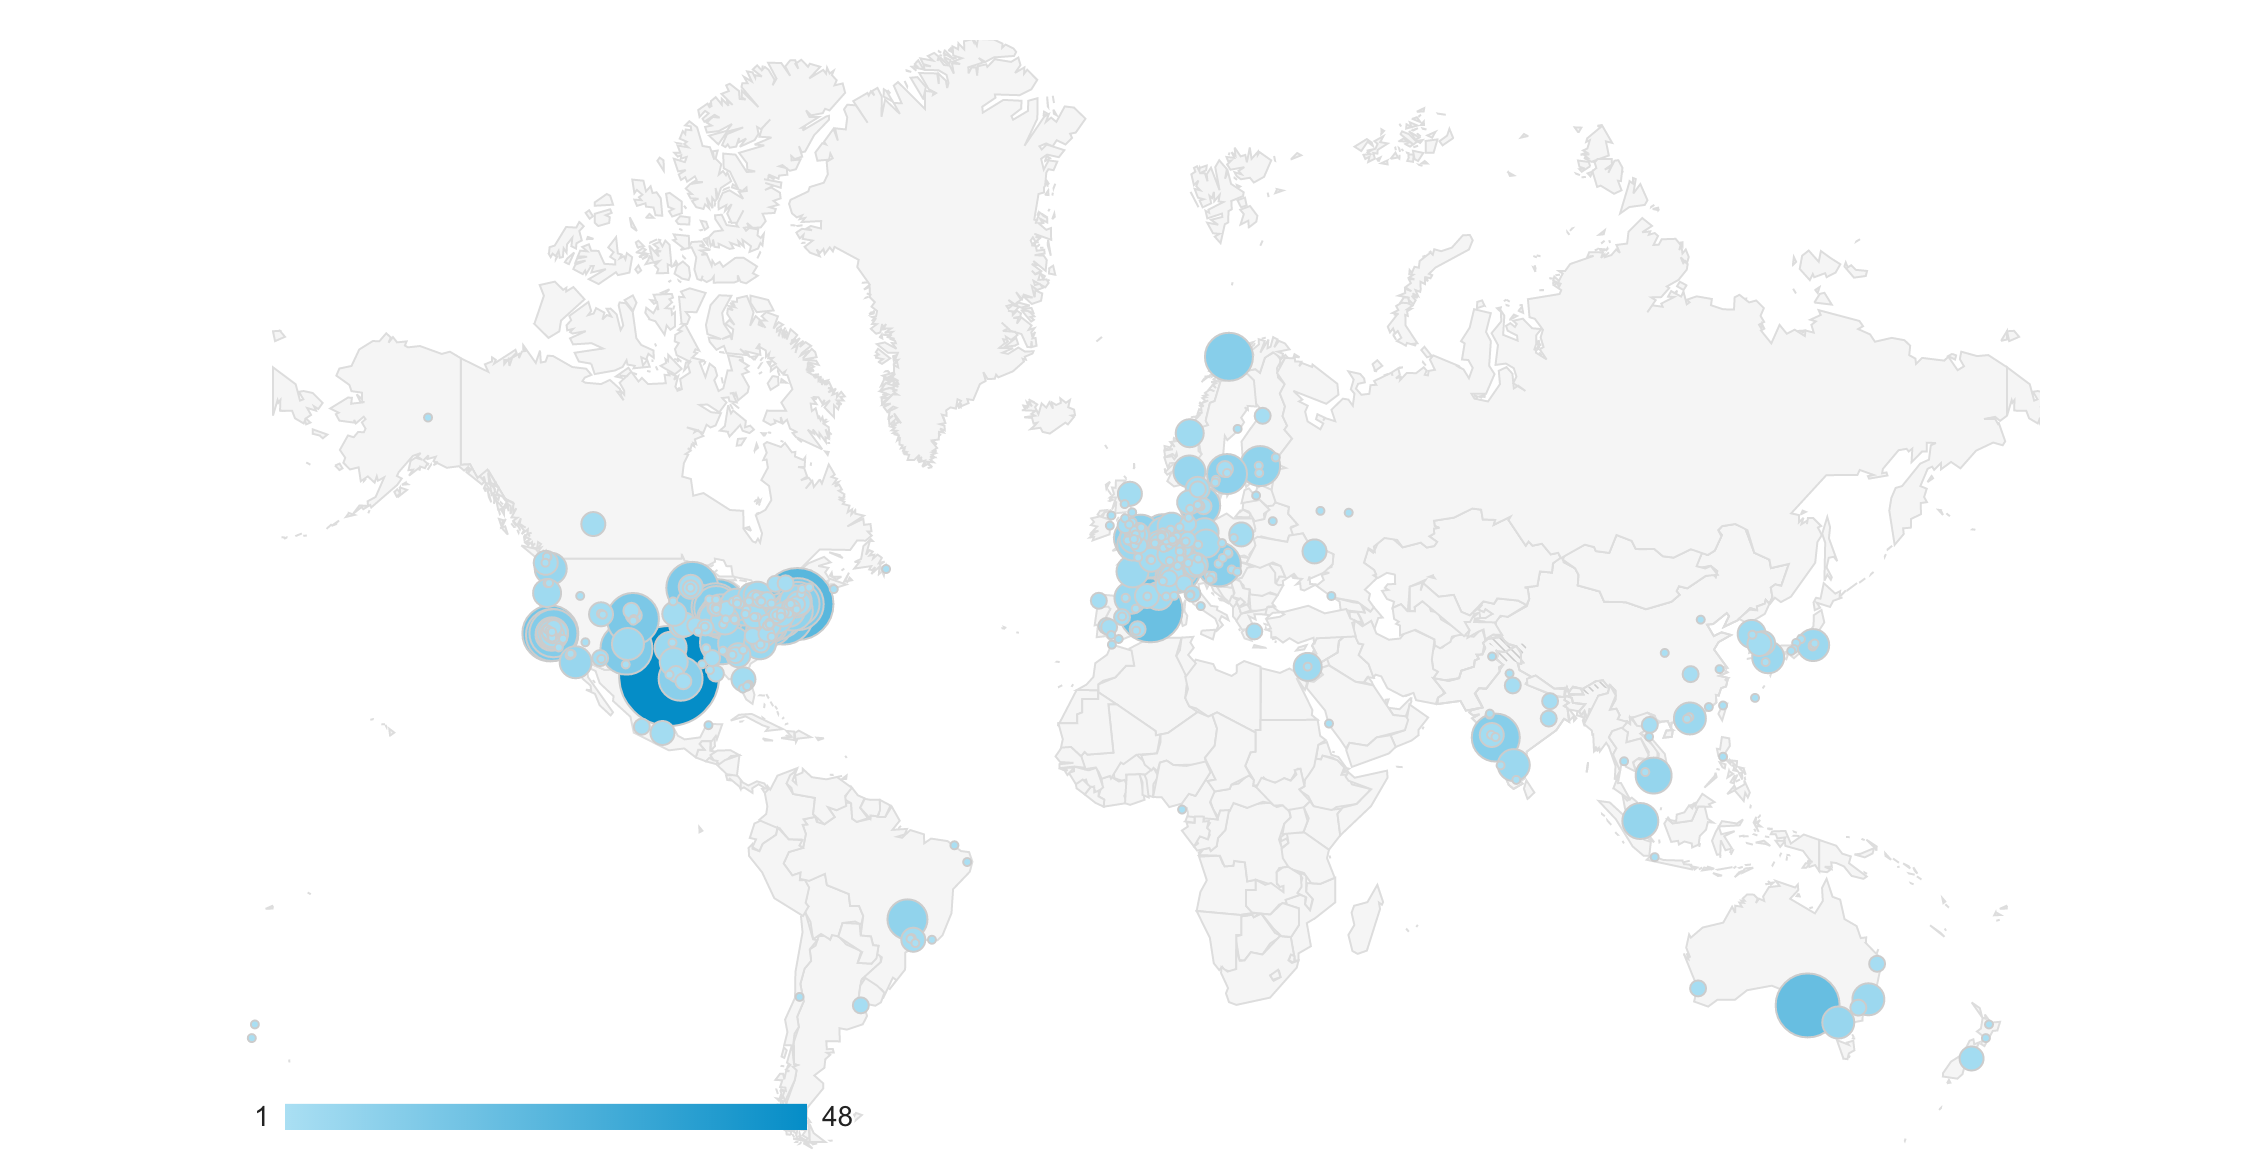
\includegraphics[width=.9\textwidth]{Lmod_doc_usage}}
\end{frame}

%page 40
\begin{frame}{Conclusions: Lmod}
  \begin{itemize}
    \item Latest version: https://github.com:TACC/Lmod.git
    \item Stable version: http://lmod.sf.net
    \item Documentation:  http://lmod.readthedocs.org
    \item Shell Startup Debug: http://shellstartupdebug.sf.net
    \item Mailing List:   lmod-users@lists.sourceforge.net.
    \item Join here: https://lists.sourceforge.net/lists/listinfo/lmod-users
  \end{itemize}
\end{frame}

\end{document}
